% book01.tex — Book I of Euclid's Elements: Plane Geometry.
%
% Each Proposition X.Y is a `claim` with the statement; its proof is
% an `evidence` block; the dependency DAG is encoded via \dependson
% edges at the close of each proof.
%
% Statement wording follows Heath (1908), public domain, with minor
% modernisation. Proof summaries are condensed for legibility; the
% point of this encoding is to make the *dependency graph*
% machine-readable, not to be a substitute for a full geometric exposition.

\section{Book I --- Plane Geometry}
\label{sec:book-I}

\begin{claim}[Proposition I.1: Equilateral triangle on a given segment]
\label{prop:I.1}
On a given finite straight line to construct an equilateral triangle.
\end{claim}

\begin{evidence}[Proof of I.1]
\label{ev:I.1}
% fig-i-1.tex — I.1: equilateral triangle on a given segment.
\begin{figure}[H]
\centering
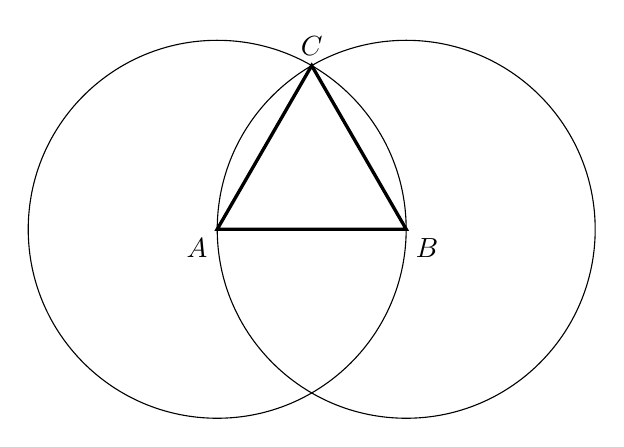
\begin{tikzpicture}[scale=1.2, line cap=round]
  \coordinate (A) at (0,0);
  \coordinate (B) at (2,0);
  \coordinate (C) at (1,{sqrt(3)});
  % Two circles, centres A and B, radius AB.
  \draw[thin] (A) circle (2);
  \draw[thin] (B) circle (2);
  % Triangle.
  \draw[very thick] (A) -- (B) -- (C) -- cycle;
  % Labels.
  \node[below left]  at (A) {$A$};
  \node[below right] at (B) {$B$};
  \node[above]       at (C) {$C$};
\end{tikzpicture}
\caption{Proposition I.1. The two circles with centres $A$ and $B$ and
common radius $AB$ meet at $C$; the triangle $ABC$ is equilateral.}
\label{fig:I.1}
\end{figure}

Let $AB$ be the given finite straight line.  With centre $A$ and
distance $AB$ describe the circle $BCD$ (Postulate 3).  With centre
$B$ and distance $BA$ describe the circle $ACE$ (Postulate 3).  From
the point $C$, where the circles cut one another, draw $CA$ and $CB$
(Postulate 1).  Since $A$ is the centre of $BCD$, $AC = AB$
(Definition I.15).  Since $B$ is the centre of $ACE$, $BC = BA$
(Definition I.15).  By Common Notion 1, $AC = BC$.  Therefore the
triangle $ABC$ is equilateral.
\dependson{I.1}{post:1}
\dependson{I.1}{post:3}
\dependson{I.1}{def:I.15}
\dependson{I.1}{cn:1}
\end{evidence}

\begin{claim}[Proposition I.2: Transfer a segment to a given point]
\label{prop:I.2}
To place at a given point (as an extremity) a straight line equal to a
given straight line.
\end{claim}
\begin{evidence}[Proof of I.2]
\label{ev:I.2}
Apply I.1 to obtain an equilateral triangle; produce its sides
(Postulate 2); describe a circle with centre at one endpoint of the
given segment cutting one of the produced sides; the cut-off equals
the given segment by Definition I.15 and Common Notion 1.
\dependson{I.2}{I.1}
\dependson{I.2}{post:1}
\dependson{I.2}{post:2}
\dependson{I.2}{post:3}
\dependson{I.2}{def:I.15}
\dependson{I.2}{cn:1}
\end{evidence}

\begin{claim}[Proposition I.3: Cut off a segment equal to a shorter]
\label{prop:I.3}
Given two unequal straight lines, to cut off from the greater a
straight line equal to the less.
\end{claim}
\begin{evidence}[Proof of I.3]
\label{ev:I.3}
Use I.2 to construct, at one extremity of the longer line, a segment
equal to the shorter.  Then by Definition I.15 the desired cut-off is
obtained.
\dependson{I.3}{I.2}
\dependson{I.3}{def:I.15}
\end{evidence}

\begin{claim}[Proposition I.4: SAS congruence]
\label{prop:I.4}
If two triangles have two sides equal to two sides respectively, and
have the angles contained by the equal straight lines equal, then they
will also have the base equal to the base, the triangle will be equal
to the triangle, and the remaining angles will be equal to the
remaining angles respectively.
\end{claim}
\begin{evidence}[Proof of I.4]
\label{ev:I.4}
Superpose one triangle on the other; corresponding sides and angles
coincide; by Common Notion 4 the figures are equal.
\dependson{I.4}{cn:4}
\end{evidence}

\begin{claim}[Proposition I.5: Pons asinorum]
\label{prop:I.5}
In isosceles triangles the angles at the base are equal to one
another; and if the equal straight lines be produced further, the
angles under the base will be equal to one another.
\end{claim}
\begin{evidence}[Proof of I.5]
\label{ev:I.5}
% fig-i-5.tex — I.5: pons asinorum (base angles of an isoceles triangle).
\begin{figure}[H]
\centering
\begin{tikzpicture}[scale=1.0, line cap=round]
  \coordinate (A) at (0, 3);
  \coordinate (B) at (-1.5, 0);
  \coordinate (C) at (1.5, 0);
  % Equal sides AB and AC, extended to F and G.
  \coordinate (F) at ($(A)!2.0!(B)$);
  \coordinate (G) at ($(A)!2.0!(C)$);
  \draw[thin]      (A) -- (F);
  \draw[thin]      (A) -- (G);
  \draw[very thick] (B) -- (C);
  % Points D on BF, E on CG with BD = CE.
  \coordinate (D) at ($(B)!0.5!(F)$);
  \coordinate (E) at ($(C)!0.5!(G)$);
  \draw[very thick, dashed] (B) -- (E);
  \draw[very thick, dashed] (C) -- (D);
  % Labels.
  \node[above]      at (A) {$A$};
  \node[left]       at (B) {$B$};
  \node[right]      at (C) {$C$};
  \node[below left] at (D) {$D$};
  \node[below right] at (E) {$E$};
  \node[below left] at (F) {$F$};
  \node[below right] at (G) {$G$};
\end{tikzpicture}
\caption{Proposition I.5. With $AB = AC$ and $BD = CE$ on the extensions,
triangles $ABE$ and $ACD$ are congruent (SAS, by I.4), whence the base
angles $\angle ABC = \angle ACB$.}
\label{fig:I.5}
\end{figure}

Apply I.3 to mark equal segments on the produced sides, then I.4 to
two pairs of congruent triangles.  Common Notion 3 gives equality of
the remaining angles.
\dependson{I.5}{I.3}
\dependson{I.5}{I.4}
\dependson{I.5}{cn:3}
\end{evidence}

\begin{claim}[Proposition I.6: Converse of I.5]
\label{prop:I.6}
If in a triangle two angles are equal to one another, the sides which
subtend the equal angles will also be equal to one another.
\end{claim}
\begin{evidence}[Proof of I.6]
\label{ev:I.6}
Suppose the sides unequal; cut off (by I.3) the greater equal to the
less; by I.4 the resulting smaller triangle equals the whole, which
contradicts Common Notion 5.  Therefore the sides are equal.
\dependson{I.6}{I.3}
\dependson{I.6}{I.4}
\dependson{I.6}{cn:5}
\end{evidence}

\begin{claim}[Proposition I.7: Uniqueness of triangle on a base]
\label{prop:I.7}
Given two straight lines constructed on a straight line and meeting in
a point, there cannot be constructed on the same straight line and on
the same side of it two other straight lines meeting in another point
and equal to the former two respectively, namely each to that which
has the same extremity with it.
\end{claim}
\begin{evidence}[Proof of I.7]
\label{ev:I.7}
A double application of I.5 yields contradictory angle equalities; by
Common Notion 5 the second meeting point cannot exist.
\dependson{I.7}{I.5}
\dependson{I.7}{cn:5}
\end{evidence}

\begin{claim}[Proposition I.8: SSS congruence]
\label{prop:I.8}
If two triangles have the two sides equal to two sides respectively,
and have also the base equal to the base, they will also have the
angles equal which are contained by the equal straight lines.
\end{claim}
\begin{evidence}[Proof of I.8]
\label{ev:I.8}
Superpose and apply I.7 to rule out a non-coincident image of the
contained angle; conclude by Common Notion 4.
\dependson{I.8}{I.7}
\dependson{I.8}{cn:4}
\end{evidence}

\begin{claim}[Proposition I.9: Angle bisection]
\label{prop:I.9}
To bisect a given rectilineal angle.
\end{claim}
\begin{evidence}[Proof of I.9]
\label{ev:I.9}
Apply I.1 to construct an equilateral triangle on a chord between the
angle's sides; the line from the vertex to the equilateral's apex
bisects the angle by I.8.
\dependson{I.9}{I.1}
\dependson{I.9}{I.8}
\end{evidence}

\begin{claim}[Proposition I.10: Segment bisection]
\label{prop:I.10}
To bisect a given finite straight line.
\end{claim}
\begin{evidence}[Proof of I.10]
\label{ev:I.10}
Apply I.1 to erect an equilateral triangle on the segment; bisect the
opposite angle by I.9; the bisector meets the segment at its midpoint
by I.4.
\dependson{I.10}{I.1}
\dependson{I.10}{I.9}
\dependson{I.10}{I.4}
\end{evidence}

\begin{claim}[Proposition I.11: Perpendicular at a point]
\label{prop:I.11}
To draw a straight line at right angles to a given straight line from
a given point on it.
\end{claim}
\begin{evidence}[Proof of I.11]
\label{ev:I.11}
Apply I.3 to mark equal segments either side of the given point, then
I.1 to erect an equilateral triangle whose apex line is perpendicular
(by I.8 and Definition I.10).
\dependson{I.11}{I.1}
\dependson{I.11}{I.3}
\dependson{I.11}{I.8}
\dependson{I.11}{def:I.10}
\end{evidence}

\begin{claim}[Proposition I.12: Perpendicular from external point]
\label{prop:I.12}
To draw a perpendicular straight line to a given infinite straight
line from a given point not on it.
\end{claim}
\begin{evidence}[Proof of I.12]
\label{ev:I.12}
With centre at the external point describe a circle (Postulate 3)
cutting the given line; bisect the chord by I.10; the line from the
external point to the midpoint is perpendicular by I.8.
\dependson{I.12}{I.8}
\dependson{I.12}{I.10}
\dependson{I.12}{post:3}
\end{evidence}

\begin{claim}[Proposition I.13: Adjacent angles sum to two right angles]
\label{prop:I.13}
If a straight line set up on a straight line make angles, it will
make either two right angles or angles equal to two right angles.
\end{claim}
\begin{evidence}[Proof of I.13]
\label{ev:I.13}
Drop a perpendicular by I.11; Common Notions 1--2 sum the resulting
two right angles to the unequal-case angle sum.
\dependson{I.13}{I.11}
\dependson{I.13}{cn:1}
\dependson{I.13}{cn:2}
\dependson{I.13}{def:I.10}
\end{evidence}

\begin{claim}[Proposition I.14: Converse of I.13]
\label{prop:I.14}
If with any straight line, and at a point on it, two straight lines
not lying on the same side make the adjacent angles equal to two
right angles, the two straight lines will be in a straight line with
one another.
\end{claim}
\begin{evidence}[Proof of I.14]
\label{ev:I.14}
Suppose not; then I.13 and Common Notion 1 yield contradictory angle
sums.
\dependson{I.14}{I.13}
\dependson{I.14}{cn:1}
\end{evidence}

\begin{claim}[Proposition I.15: Vertical angles]
\label{prop:I.15}
If two straight lines cut one another, they make the vertical angles
equal to one another.
\end{claim}
\begin{evidence}[Proof of I.15]
\label{ev:I.15}
Apply I.13 twice and Common Notion 3.
\dependson{I.15}{I.13}
\dependson{I.15}{cn:3}
\end{evidence}

\begin{claim}[Proposition I.16: Exterior angle of a triangle]
\label{prop:I.16}
In any triangle, if one of the sides be produced, the exterior angle
is greater than either of the interior and opposite angles.
\end{claim}
\begin{evidence}[Proof of I.16]
\label{ev:I.16}
Bisect a side by I.10; produce a median; apply I.4 to obtain a
congruent triangle that has the interior angle as one of its parts;
Common Notion 5 closes the inequality.
\dependson{I.16}{I.4}
\dependson{I.16}{I.10}
\dependson{I.16}{cn:5}
\end{evidence}

\begin{claim}[Proposition I.17: Sum of any two angles $<$ two right angles]
\label{prop:I.17}
In any triangle two angles taken together in any manner are less than
two right angles.
\end{claim}
\begin{evidence}[Proof of I.17]
\label{ev:I.17}
Apply I.16 and I.13.
\dependson{I.17}{I.13}
\dependson{I.17}{I.16}
\end{evidence}

\begin{claim}[Proposition I.18: Greater side subtends greater angle]
\label{prop:I.18}
In any triangle the greater side subtends the greater angle.
\end{claim}
\begin{evidence}[Proof of I.18]
\label{ev:I.18}
Cut off (I.3) a segment on the greater side equal to the lesser;
apply I.5 and I.16.
\dependson{I.18}{I.3}
\dependson{I.18}{I.5}
\dependson{I.18}{I.16}
\end{evidence}

\begin{claim}[Proposition I.19: Converse of I.18]
\label{prop:I.19}
In any triangle the greater angle is subtended by the greater side.
\end{claim}
\begin{evidence}[Proof of I.19]
\label{ev:I.19}
Suppose not; by I.5 and I.18 contradiction.
\dependson{I.19}{I.5}
\dependson{I.19}{I.18}
\end{evidence}

\begin{claim}[Proposition I.20: Triangle inequality]
\label{prop:I.20}
In any triangle two sides taken together in any manner are greater
than the remaining one.
\end{claim}
\begin{evidence}[Proof of I.20]
\label{ev:I.20}
Produce one side to an isosceles configuration by I.3; apply I.5 and
I.19.
\dependson{I.20}{I.3}
\dependson{I.20}{I.5}
\dependson{I.20}{I.19}
\end{evidence}

\begin{claim}[Proposition I.21: Interior cevian inequalities]
\label{prop:I.21}
If on one of the sides of a triangle, from its extremities, there be
constructed two straight lines meeting within the triangle, the
straight lines so constructed will be less than the remaining two
sides of the triangle, but will contain a greater angle.
\end{claim}
\begin{evidence}[Proof of I.21]
\label{ev:I.21}
Two applications of I.20 and one of I.16.
\dependson{I.21}{I.16}
\dependson{I.21}{I.20}
\end{evidence}

\begin{claim}[Proposition I.22: Triangle from three given segments]
\label{prop:I.22}
Out of three straight lines, which are equal to three given straight
lines, to construct a triangle: thus it is necessary that two of the
straight lines taken together in any manner should be greater than the
remaining one.
\end{claim}
\begin{evidence}[Proof of I.22]
\label{ev:I.22}
Apply I.20 (the necessity), then I.3 and Postulate 3 (the
construction).
\dependson{I.22}{I.3}
\dependson{I.22}{I.20}
\dependson{I.22}{post:3}
\end{evidence}

\begin{claim}[Proposition I.23: Reproduce a given angle]
\label{prop:I.23}
On a given straight line and at a point on it to construct a
rectilineal angle equal to a given rectilineal angle.
\end{claim}
\begin{evidence}[Proof of I.23]
\label{ev:I.23}
Cut equal segments by I.3, construct the matching triangle by I.22,
apply I.8.
\dependson{I.23}{I.3}
\dependson{I.23}{I.8}
\dependson{I.23}{I.22}
\end{evidence}

\begin{claim}[Proposition I.24: Hinge inequality]
\label{prop:I.24}
If two triangles have the two sides equal to two sides respectively,
but have the one of the angles contained by the equal straight lines
greater than the other, they will also have the base greater than the
base.
\end{claim}
\begin{evidence}[Proof of I.24]
\label{ev:I.24}
Apply I.23, I.4, I.5, and I.19.
\dependson{I.24}{I.4}
\dependson{I.24}{I.5}
\dependson{I.24}{I.19}
\dependson{I.24}{I.23}
\end{evidence}

\begin{claim}[Proposition I.25: Converse of I.24]
\label{prop:I.25}
If two triangles have the two sides equal to two sides respectively,
but have the one base greater than the other, they will also have the
one angle contained by the equal straight lines greater than the
other.
\end{claim}
\begin{evidence}[Proof of I.25]
\label{ev:I.25}
Suppose not and use I.4, I.24.
\dependson{I.25}{I.4}
\dependson{I.25}{I.24}
\end{evidence}

\begin{claim}[Proposition I.26: ASA / AAS congruence]
\label{prop:I.26}
If two triangles have the two angles equal to two angles respectively,
and one side equal to one side, namely either the side adjoining the
equal angles or that subtending one of the equal angles, they will
also have the remaining sides equal to the remaining sides and the
remaining angle equal to the remaining angle.
\end{claim}
\begin{evidence}[Proof of I.26]
\label{ev:I.26}
Apply I.4 to the congruent angle--side--angle case; for the AAS case
combine I.4 with I.16.
\dependson{I.26}{I.4}
\dependson{I.26}{I.16}
\end{evidence}

\begin{claim}[Proposition I.27: Alternate angles imply parallels]
\label{prop:I.27}
If a straight line falling on two straight lines make the alternate
angles equal to one another, the straight lines will be parallel to
one another.
\end{claim}
\begin{evidence}[Proof of I.27]
\label{ev:I.27}
Suppose the lines meet; I.16 gives a contradiction.  By Definition
I.23 they are parallel.
\dependson{I.27}{I.16}
\dependson{I.27}{def:I.23}
\end{evidence}

\begin{claim}[Proposition I.28: Corresponding angles imply parallels]
\label{prop:I.28}
If a straight line falling on two straight lines make the exterior
angle equal to the interior and opposite angle on the same side, or
the interior angles on the same side equal to two right angles, the
straight lines will be parallel to one another.
\end{claim}
\begin{evidence}[Proof of I.28]
\label{ev:I.28}
Reduce to I.27 via I.13 and I.15.
\dependson{I.28}{I.13}
\dependson{I.28}{I.15}
\dependson{I.28}{I.27}
\end{evidence}

\begin{claim}[Proposition I.29: Properties of parallels (uses Postulate 5)]
\label{prop:I.29}
A straight line falling on parallel straight lines makes the alternate
angles equal to one another, the exterior angle equal to the interior
and opposite angle, and the interior angles on the same side equal to
two right angles.
\end{claim}
\begin{evidence}[Proof of I.29]
\label{ev:I.29}
The first use of Postulate 5: any contrary supposition contradicts the
parallel postulate via I.13.
\dependson{I.29}{I.13}
\dependson{I.29}{post:5}
\end{evidence}

\begin{claim}[Proposition I.30: Transitivity of parallelism]
\label{prop:I.30}
Straight lines parallel to the same straight line are also parallel
to one another.
\end{claim}
\begin{evidence}[Proof of I.30]
\label{ev:I.30}
Two applications of I.29 and Common Notion 1.
\dependson{I.30}{I.29}
\dependson{I.30}{cn:1}
\end{evidence}

\begin{claim}[Proposition I.31: Construct a parallel through a point]
\label{prop:I.31}
Through a given point to draw a straight line parallel to a given
straight line.
\end{claim}
\begin{evidence}[Proof of I.31]
\label{ev:I.31}
Apply I.23 to reproduce the alternate angle at the given point and
I.27 to conclude parallelism.
\dependson{I.31}{I.23}
\dependson{I.31}{I.27}
\end{evidence}

\begin{claim}[Proposition I.32: Triangle angle sum]
\label{prop:I.32}
In any triangle, if one of the sides be produced, the exterior angle
is equal to the two interior and opposite angles, and the three
interior angles of the triangle are equal to two right angles.
\end{claim}
\begin{evidence}[Proof of I.32]
% fig-i-32.tex — I.32: triangle angle sum (parallel through apex).
\begin{figure}[H]
\centering
\begin{tikzpicture}[scale=1.2, line cap=round]
  \coordinate (A) at (-1.5, 0);
  \coordinate (B) at (2.0, 0);
  \coordinate (C) at (0.5, 2.4);
  \coordinate (D) at ($(C)!-1.4!(A)$); % line through C parallel to AB, on left
  \coordinate (E) at ($(C)!-1.4!(B)$); % line through C parallel to AB, on right
  % Triangle.
  \draw[very thick] (A) -- (B) -- (C) -- cycle;
  % Parallel through C, drawn long.
  \draw[thin] ($(C)!-0.7!(B)$) -- ($(C)!1.5!(B)$);
  % Side AB extended beyond B to F to expose exterior angle.
  \coordinate (F) at ($(A)!1.4!(B)$);
  \draw[thin] (B) -- (F);
  % Labels.
  \node[below left]  at (A) {$A$};
  \node[below right] at (B) {$B$};
  \node[above]       at (C) {$C$};
  \node[below right] at (F) {$F$};
  \node[above left]  at ($(C)!-0.7!(B)$) {$D$};
  \node[above right] at ($(C)!1.5!(B)$) {$E$};
\end{tikzpicture}
\caption{Proposition I.32. Drawing $DE$ through $C$ parallel to $AB$
makes $\angle DCA = \angle CAB$ (alternate, I.29) and $\angle ECB =
\angle ABC$ (alternate, I.29); the straight angle at $C$ then sums
the three interior angles of $\triangle ABC$ to two right angles.}
\label{fig:I.32}
\end{figure}

\label{ev:I.32}
Apply I.31 to draw a parallel through the apex; apply I.29 twice and
Common Notion 2.
\dependson{I.32}{I.29}
\dependson{I.32}{I.31}
\dependson{I.32}{cn:2}
\end{evidence}

\begin{claim}[Proposition I.33: Connecting equal-and-parallel pairs]
\label{prop:I.33}
The straight lines joining equal and parallel straight lines (at the
extremities which are in the same directions) are themselves equal
and parallel.
\end{claim}
\begin{evidence}[Proof of I.33]
\label{ev:I.33}
Apply I.4 to the resulting two triangles and I.29 + I.27 for
parallelism.
\dependson{I.33}{I.4}
\dependson{I.33}{I.27}
\dependson{I.33}{I.29}
\end{evidence}

\begin{claim}[Proposition I.34: Properties of parallelograms]
\label{prop:I.34}
In parallelogrammic areas the opposite sides and angles are equal to
one another, and the diameter bisects the areas.
\end{claim}
\begin{evidence}[Proof of I.34]
\label{ev:I.34}
Apply I.29 and I.26 to the two triangles cut by the diameter, then
Common Notion 2.
\dependson{I.34}{I.26}
\dependson{I.34}{I.29}
\dependson{I.34}{cn:2}
\end{evidence}

\begin{claim}[Proposition I.35: Parallelograms with same base \& between same parallels]
\label{prop:I.35}
Parallelograms which are on the same base and in the same parallels
are equal to one another.
\end{claim}
\begin{evidence}[Proof of I.35]
\label{ev:I.35}
Apply I.34 and I.4 to congruent triangles; conclude by Common Notions
2--3.
\dependson{I.35}{I.4}
\dependson{I.35}{I.34}
\dependson{I.35}{cn:2}
\dependson{I.35}{cn:3}
\end{evidence}

\begin{claim}[Proposition I.36: Parallelograms with equal bases]
\label{prop:I.36}
Parallelograms which are on equal bases and in the same parallels are
equal to one another.
\end{claim}
\begin{evidence}[Proof of I.36]
\label{ev:I.36}
Translate one parallelogram via I.33 to share a base with the other,
then apply I.35.
\dependson{I.36}{I.33}
\dependson{I.36}{I.35}
\end{evidence}

\begin{claim}[Proposition I.37: Triangles with same base \& parallels]
\label{prop:I.37}
Triangles which are on the same base and in the same parallels are
equal to one another.
\end{claim}
\begin{evidence}[Proof of I.37]
\label{ev:I.37}
Complete each triangle to a parallelogram via I.31, then apply I.34
and I.35.
\dependson{I.37}{I.31}
\dependson{I.37}{I.34}
\dependson{I.37}{I.35}
\end{evidence}

\begin{claim}[Proposition I.38: Triangles with equal bases]
\label{prop:I.38}
Triangles which are on equal bases and in the same parallels are
equal to one another.
\end{claim}
\begin{evidence}[Proof of I.38]
\label{ev:I.38}
Same construction as I.37 with I.36 in place of I.35.
\dependson{I.38}{I.31}
\dependson{I.38}{I.34}
\dependson{I.38}{I.36}
\end{evidence}

\begin{claim}[Proposition I.39: Equal triangles on same base $\Rightarrow$ same parallels]
\label{prop:I.39}
Equal triangles which are on the same base and on the same side are
also in the same parallels.
\end{claim}
\begin{evidence}[Proof of I.39]
\label{ev:I.39}
Apply I.31 to draw a parallel; I.37 forces the second vertex onto it.
\dependson{I.39}{I.31}
\dependson{I.39}{I.37}
\end{evidence}

\begin{claim}[Proposition I.40: Equal triangles on equal bases]
\label{prop:I.40}
Equal triangles which are on equal bases and on the same side are
also in the same parallels.
\end{claim}
\begin{evidence}[Proof of I.40]
\label{ev:I.40}
Same approach as I.39 with I.38 in place of I.37.
\dependson{I.40}{I.31}
\dependson{I.40}{I.38}
\end{evidence}

\begin{claim}[Proposition I.41: Parallelogram is double a triangle]
\label{prop:I.41}
If a parallelogram have the same base with a triangle and be in the
same parallels, the parallelogram is double of the triangle.
\end{claim}
\begin{evidence}[Proof of I.41]
\label{ev:I.41}
Apply I.34 and I.37; double via Common Notion 2.
\dependson{I.41}{I.34}
\dependson{I.41}{I.37}
\dependson{I.41}{cn:2}
\end{evidence}

\begin{claim}[Proposition I.42: Construct a parallelogram equal in area to a triangle]
\label{prop:I.42}
To construct, in a given rectilineal angle, a parallelogram equal to
a given triangle.
\end{claim}
\begin{evidence}[Proof of I.42]
\label{ev:I.42}
Bisect a side by I.10; apply I.23 to set the angle; apply I.31 and
I.41.
\dependson{I.42}{I.10}
\dependson{I.42}{I.23}
\dependson{I.42}{I.31}
\dependson{I.42}{I.41}
\end{evidence}

\begin{claim}[Proposition I.43: Complements of a parallelogram]
\label{prop:I.43}
In any parallelogram the complements of the parallelograms about the
diameter are equal to one another.
\end{claim}
\begin{evidence}[Proof of I.43]
\label{ev:I.43}
Apply I.34 to the bisecting diameter and Common Notions 2--3.
\dependson{I.43}{I.34}
\dependson{I.43}{cn:2}
\dependson{I.43}{cn:3}
\end{evidence}

\begin{claim}[Proposition I.44: Apply a parallelogram to a segment equal to a triangle]
\label{prop:I.44}
To a given straight line to apply, in a given rectilineal angle, a
parallelogram equal to a given triangle.
\end{claim}
\begin{evidence}[Proof of I.44]
\label{ev:I.44}
Apply I.42 and I.43 in sequence.
\dependson{I.44}{I.42}
\dependson{I.44}{I.43}
\end{evidence}

\begin{claim}[Proposition I.45: Apply a parallelogram equal to a rectilineal figure]
\label{prop:I.45}
To construct, in a given rectilineal angle, a parallelogram equal to
a given rectilineal figure.
\end{claim}
\begin{evidence}[Proof of I.45]
\label{ev:I.45}
Triangulate the figure; sum the parallelograms by repeated I.44 and
Common Notion 2.
\dependson{I.45}{I.44}
\dependson{I.45}{cn:2}
\end{evidence}

\begin{claim}[Proposition I.46: Construct a square on a segment]
\label{prop:I.46}
On a given straight line to describe a square.
\end{claim}
\begin{evidence}[Proof of I.46]
\label{ev:I.46}
Apply I.11 to erect perpendiculars; use I.3 to cut off equal segments;
use I.31 and I.29 to close the square; verify right angles via I.34.
\dependson{I.46}{I.3}
\dependson{I.46}{I.11}
\dependson{I.46}{I.29}
\dependson{I.46}{I.31}
\dependson{I.46}{I.34}
\end{evidence}

\begin{claim}[Proposition I.47: Pythagoras' theorem]
\label{prop:I.47}
In right-angled triangles the square on the side subtending the right
angle is equal to the squares on the sides containing the right angle.
\end{claim}
\begin{evidence}[Proof of I.47]
% fig-i-47.tex — I.47: Pythagoras (square decomposition).
\begin{figure}[H]
\centering
\begin{tikzpicture}[scale=0.55, line cap=round, line join=round]
  % Right triangle vertices: right angle at A.
  \coordinate (A) at (0, 0);
  \coordinate (B) at (3, 0); % horizontal leg
  \coordinate (C) at (0, 4); % vertical leg
  % Hypotenuse BC.
  % Square on AB (below): A, B, B', A'
  \coordinate (Ap) at (0, -3);
  \coordinate (Bp) at (3, -3);
  % Square on AC (left): A, C, C', A''
  \coordinate (App) at (-4, 0);
  \coordinate (Cp)  at (-4, 4);
  % Square on BC (outward): B, C, C'', B''
  % Outward direction = rotate (B-C) by -90.
  \coordinate (Bpp) at ($(B)!1!-90:(C)$);
  \coordinate (Cpp) at ($(C)!1!90:(B)$);
  % Triangle.
  \draw[very thick] (A) -- (B) -- (C) -- cycle;
  % Three squares.
  \draw[thick, fill=gray!10] (A)   -- (B)   -- (Bp)  -- (Ap)  -- cycle;
  \draw[thick, fill=gray!10] (A)   -- (C)   -- (Cp)  -- (App) -- cycle;
  \draw[thick, fill=gray!20] (B)   -- (C)   -- (Cpp) -- (Bpp) -- cycle;
  % Altitude from A to BC, foot at H, extended to meet square on BC.
  \coordinate (H) at ($(B)!(A)!(C)$);
  \coordinate (Hext) at ($(H)!1!-90:(B)$);
  \draw[thin, dashed] (A) -- (Hext);
  % Labels.
  \node[below right]      at (A) {$A$};
  \node[below]            at (B) {$B$};
  \node[left]             at (C) {$C$};
  \node[left]             at ($(A)!0.5!(App)$) {square on $AC$};
  \node                   at ($(A)!0.5!(Bp)+(0.5,-1.5)$) {square on $AB$};
  \node                   at ($(B)!0.5!(Cpp)+(1.7,0.7)$) {square on $BC$};
\end{tikzpicture}
\caption{Proposition I.47. The square on the hypotenuse $BC$ is
partitioned by the altitude $AH$ extended into two rectangles, each
equal (by I.41 + I.46) to a square on a leg; thus $BC^2 = AB^2 + AC^2$.}
\label{fig:I.47}
\end{figure}

\label{ev:I.47}
Erect squares on each side via I.46; using I.14, I.31 and I.41 show
each part-square equals a corresponding parallelogram cut off the
hypotenuse-square by the perpendicular from the right angle; sum via
Common Notion 2.
\dependson{I.47}{I.4}
\dependson{I.47}{I.14}
\dependson{I.47}{I.31}
\dependson{I.47}{I.41}
\dependson{I.47}{I.46}
\dependson{I.47}{cn:2}
\supports{I.47}{I.48}
\end{evidence}

\begin{claim}[Proposition I.48: Converse of Pythagoras]
\label{prop:I.48}
If in a triangle the square on one of the sides be equal to the
squares on the remaining two sides of the triangle, the angle
contained by the remaining two sides of the triangle is right.
\end{claim}
\begin{evidence}[Proof of I.48]
\label{ev:I.48}
Construct a right triangle with the same two legs by I.11; apply
I.47, I.8, and Common Notion 1.
\dependson{I.48}{I.8}
\dependson{I.48}{I.11}
\dependson{I.48}{I.47}
\dependson{I.48}{cn:1}
\end{evidence}
